%% Karlsruhe Institute of Technology
%% Institute for Anthropomatics and Robotics (IAR)
%% Artificial Intelligence for Language Technologies (AI4LT) lab
%%
%% Prof. Dr. Jan Niehues
%% Lab's website https://ai4lt.anthropomatik.kit.edu/english/index.php

\chapter{Evaluation}
\label{ch:Evaluation}
The evaluation of results of the experiments that were concucted on the benchmark section of the IWSLT 2023 dataset \cite{sperber2024evaluating} with regards to \ref{ch:Dataset}

pearson correlate \cite{2020SciPy-NMeth} the results to comet scores and compare those 
\todo{maybe move evaluations metrics here?}
%% -------------------
%% | Example content |
%% -------------------


\section{Transcription evaluation}

using WER\ref{wer}, proposed in \cite{woodard1982} and \cite{morris2004}, as reference score to compare the transctiption quality estimation metric by correlating the wer scores with the help of the pearsoncorrelation \cite{2020SciPy-NMeth}
As WER is case sensitive, both the model result and the reference are normalised to be all lowercase, as the capialisation should have no effect on the quality of the the transcription
\todo{add (scatter)plot with model and reference prob plotted, expand}
\begin{figure}
    \centering
    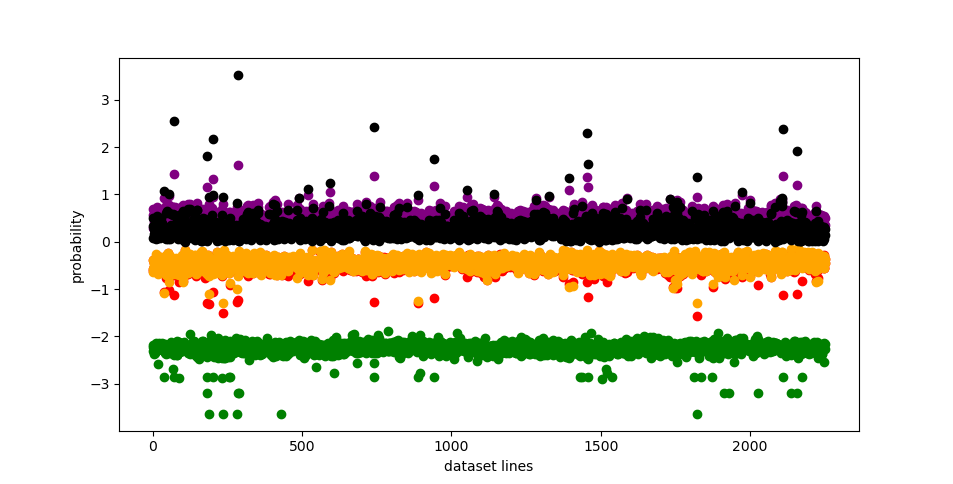
\includegraphics[width=0.5\linewidth]{Latex/sections/images/dlm plot.png}
    \caption{plot over the transctiption proabilites, the transcription means and the WER scores}
    \label{fig:transcript scatter plot}
\end{figure}

\section{Translation evaluation}

generate reference score with the help of comet \cite{rei-etal-2020-comet} which means that a score close to 1 is a good translation and a score close to 0 is a bad translation that is no better than random chance.
those reference scores are then also pearson correlated with the scores from the model. 
\begin{figure}
    \centering
    \includegraphics[width=0.5\linewidth]{images/translationcatterpolot.png}
    \caption{Plot over the translation probabilities and the reference scores}
    \label{fig:translationeval scatter plot}
\end{figure}
\todo{add (scatter)plot, expand, compare results from seamless to dlm and the end to end scores}

\section{Dropout evaluation}
the dropout score is calculated by taking the mean of the dropout probabilities of the model, the variance of the dropout probabilities and a combination of both, the dropout score is then pearson correlated with the comet scores or the word error scores in the case of the transctiption. 
for this the dropout probabilities are calculated by running the model 30 times with the dropout layer enabled and then taking the mean and variance of the resulting probabilities. 
\todo{add text, explain results, compare them, add scatter plot}

\begin{figure}
    \centering
    \includegraphics[width=0.5\linewidth]{images/dropoutscatterplot.png}
    \caption{plot over the dropout translation probabilites, the variances and the references}
    \label{fig:dropout scatter plot}
\end{figure}

\section{One unified score}
since several different metrics are used in the translation part of the cascaded model it is interesting which one might be the best choice to use in a unified score, from the text translation paper \cite{fomicheva2020unsupervised} we can gather that different metrics work better for different language groups, as this thesis only tested on english to german translation no definite choice can be made but

\todo{expand, add full judgement}
for a unified score the baselines, which are the tranlsation and transcription probability, are multiplied
but considering the results it might be better to use \todo{fill out}

\section{Pearsoncorrelation scores}
\begin{table}[ht]
  \begin{tabular}
  {l|llll}
  &  Whisper \\ \hline
  Transcription Probability& -0.33164 \\
  Transription mean & -0.60496 \\ \hline
  Dropout transcription & -0.27601 \\
  dropout variance &  \\
  \end{tabular}
  \label{transcription results}
  \caption{result from the transcription part of the cascaded model, correlatated with WER scores, with the reference and model transcript normalized}
\end{table}

\begin{table}[ht]
\begin{tabular}{l|llll}
    & Seamless & $\Delta$LM&  Seamless e2e\\ \hline
Translation & 0.37592 & 0.28284 & 0.656299\\ 
Softmax Entropy & -0.30604   & 0.083771 or  0.18071 & -0.60334 \\
Standard deviation & -0.32905  & -0.25363& -0.67148 \\ \hline

Dropout translation & 0.149888 & 0.282556& 0.14194\\

Dropout Variance &-0.10637 & -0.16285& 0.13080\\
Dropout combo & -0.163593& 0.17962061& -0.20624\\
\hline
unified score   &  &  & - 
%{transcription'pearsonr': -0.3258220972065334} transcription mean {'pearsonr': -0.27601804379827566}

%dlm probabilitycorrelation {'pearsonr': 0.2828435783527934} softmaxcorrelation {'pearsonr': 0.08377165154268117} std correlation {'pearsonr': -0.2536297836740317} dp prob corr {'pearsonr': 0.2825563734152303} dp var corr {'pearsonr': -0.1628538934576183} dpcombo {'pearsonr': 0.17962061402392054}
%seamless dropout {'pearsonr': 0.08839374531318331} {'pearsonr': -0.0962085313546643}  
\end{tabular}
\label{results}
\caption{Correlation scores for the seperate models and calculated quality scores}
\end{table}
